% Provenance (never printed): cycle 4 SVT, "La planete Terre": earthquakes,
% faults, seismic waves and their recording, magnitude and intensity, the
% link with plate boundaries; natural hazards (tsunamis) and prevention; see
% sources/book1/PROVENANCE.md. Book 1, grade 7, chapter 3.
% Vocabulary guard: P and S waves are named in prose only (they were named in
% g6.4, defined in Book 2 g11); "sediment" not before g7.4; "intensity" is
% always the earthquake's (homograph with physics: linker STOP list).
\chapter{Aardbevingen}\label{ch:g7:earthquakes}

Op de ochtend van 26~december 2004 brak onder de \omterm{def:g2:water-on-earth:ocean}{zee} voor de
noordwestpunt van Sumatra, in Indonesië, het \omterm{def:g3:stones-pebbles-sand:rock}{gesteente} langs een \omterm{def:g7:earthquakes:fault}{breuk}: het
was een van de grootste \omterm{def:g4:volcanoes-earthquakes-first-look:earthquake}{aardbevingen} die ooit zijn gemeten. Aan de nabije
\omterm{def:g1:landscapes-around-us:water}{kust} van Sumatra rees de \omterm{def:g2:water-on-earth:ocean}{zee} op in golven tot \qty{51}{m} hoog, die tot
\qty{5}{km} landinwaarts spoelden. In de uren daarna staken de golven de
Indische \omterm{def:g2:water-on-earth:ocean}{Oceaan} over en troffen ze de \omterm{def:g1:landscapes-around-us:water}{kusten} van vijftien landen, tot in
Afrika toe. Ongeveer 230\,000 mensen kwamen om. Er was toen nog geen
waarschuwingssysteem in de Indische \omterm{def:g2:water-on-earth:ocean}{Oceaan}.
% ledger: usgs:largest, nws:tsunami-2004

\begin{omfigure}
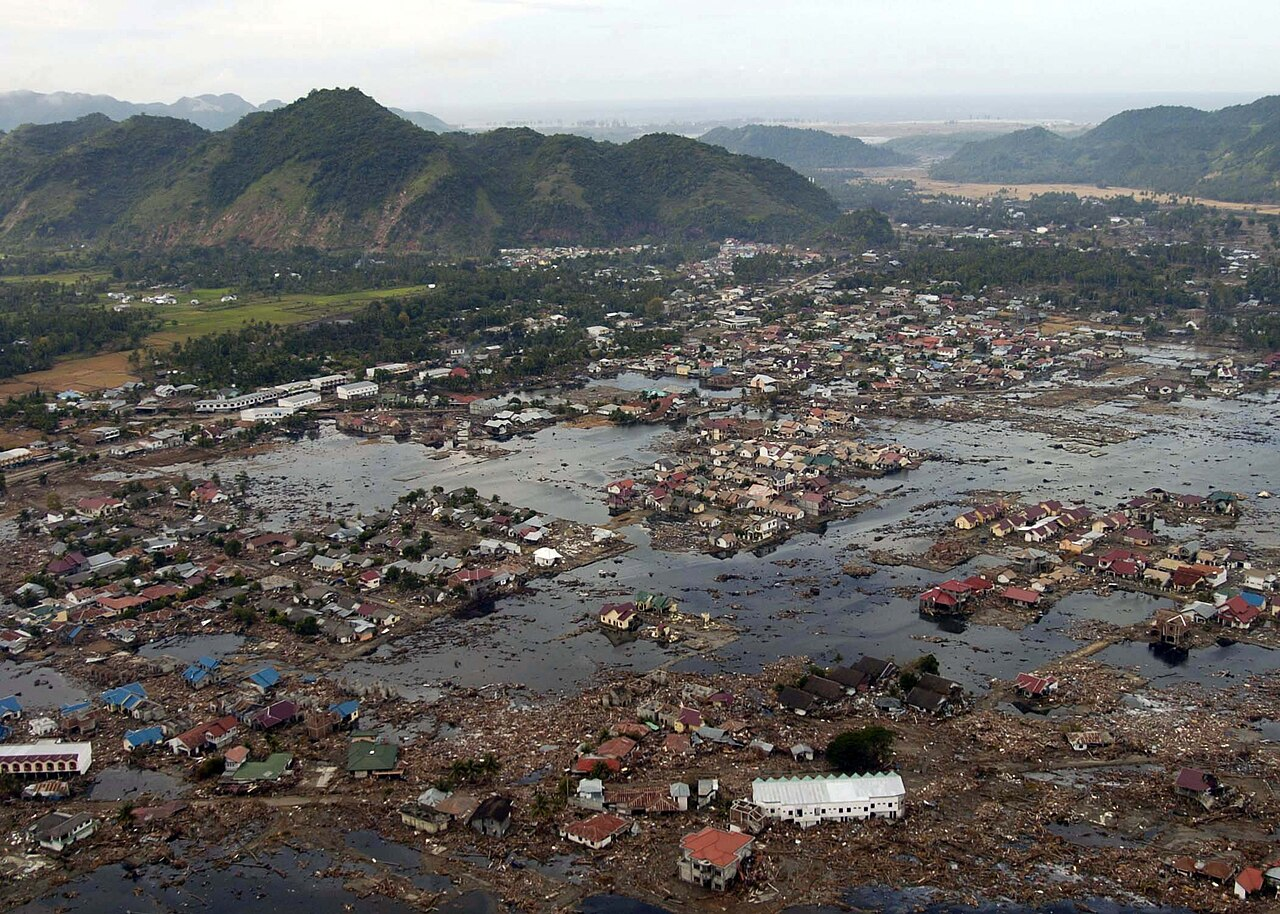
\includegraphics[width=0.78\linewidth]{images/book1/g7-tsunami-village.jpg}

{\small Een dorp bij de \omterm{def:g1:landscapes-around-us:water}{kust} van Sumatra, een week na de \omterm{def:g7:earthquakes:tsunami}{tsunami} van
26~december 2004. Foto van de U.S. Navy door Philip~A. McDaniel (publiek
domein, via Wikimedia Commons).}
% ledger: commons:tsunami-village
\label{fig:g7:earthquakes:tsunami-village}
\end{omfigure}

Hoe breekt \omterm{def:g3:stones-pebbles-sand:rock}{gesteente}? Hoe vinden wetenschappers binnen enkele minuten waar
een \omterm{def:g4:volcanoes-earthquakes-first-look:earthquake}{aardbeving} toesloeg en hoe groot ze was? En waarom rees de \omterm{def:g2:water-on-earth:ocean}{zee} uren
later op \omterm{def:g1:landscapes-around-us:water}{kusten} waar niemand iets had gevoeld?

\begin{recall}
Een \emph{\omterm{def:g4:volcanoes-earthquakes-first-look:earthquake}{aardbeving}} is een plotseling schudden van de grond, veroorzaakt
door \omterm{def:g3:stones-pebbles-sand:rock}{gesteente} dat diep onder de grond breekt en verschuift
(\cref{ch:g4:volcanoes-earthquakes-first-look}). De buitenste schil van de
Aarde bestaat uit \omterm{def:g7:plate-tectonics:plate}{platen}, en 92~\% van de grote \omterm{def:g4:volcanoes-earthquakes-first-look:earthquake}{aardbevingen} vindt plaats
op minder dan \qty{300}{km} van een \omterm{def:g7:plate-tectonics:plate-boundary}{plaatgrens}
(\cref{ch:g7:plate-tectonics}). Als een \omterm{def:g4:volcanoes-earthquakes-first-look:earthquake}{aardbeving} toeslaat, reizen er
golven door het \omterm{def:g3:stones-pebbles-sand:rock}{gesteente} van de hele Aarde: een snellere soort (de
P-golven) en een tragere soort (de S-golven); door hun aankomsttijden te
meten, ontdekten wetenschappers de \omterm{def:g6:inside-the-earth:layers}{kern} (\cref{ch:g6:inside-the-earth}).
\end{recall}

\section{Gesteente dat breekt}

De \omterm{def:g7:plate-tectonics:plate}{platen} bewegen een paar centimeter per jaar, maar hun randen zijn ruw:
ze haken in elkaar terwijl de rest van de \omterm{def:g7:plate-tectonics:plate}{platen} blijft bewegen. Het
\omterm{def:g3:stones-pebbles-sand:rock}{gesteente} bij de rand buigt een beetje door, zoals een liniaal die je aan
beide uiteinden indrukt, en slaat energie op. Als de duw uiteindelijk de
wrijving overwint, schiet het \omterm{def:g3:stones-pebbles-sand:rock}{gesteente} in één keer los en verschuift het:
die plotselinge verschuiving is de \omterm{def:g4:volcanoes-earthquakes-first-look:earthquake}{aardbeving}.
% ledger: usgs:eq-basics

\begin{definition}[Breuk]\label{def:g7:earthquakes:fault}
Een \emph{breuk}\index{breuk} is een scheur in het \omterm{def:g3:stones-pebbles-sand:rock}{gesteente} waarlangs de
twee blokken aan weerszijden ten opzichte van elkaar zijn verschoven.
Tijdens een \omterm{def:g4:volcanoes-earthquakes-first-look:earthquake}{aardbeving} schuiven de blokken plotseling langs de breuk; hoe
groter de breuk en de verschuiving, hoe groter de \omterm{def:g4:volcanoes-earthquakes-first-look:earthquake}{aardbeving}.
\end{definition}

Een \omterm{def:g7:plate-tectonics:plate-boundary}{plaatgrens} bestaat uit veel \omterm{def:g7:earthquakes:fault}{breuken}, en de meeste \omterm{def:g4:volcanoes-earthquakes-first-look:earthquake}{aardbevingen} ter
wereld vinden daarop plaats. Maar er zijn ook \omterm{def:g7:earthquakes:fault}{breuken} binnen de \omterm{def:g7:plate-tectonics:plate}{platen}, en
ook daarvan kunnen sommige plotseling verschuiven. Als een grote \omterm{def:g7:earthquakes:fault}{breuk}
dicht bij het oppervlak verschuift, is de verschuiving op de grond te zien:
een trede in een akker, een weg die in tweeën is gesneden, een hek of een
rij bomen die zijwaarts is verschoven.
% ledger: usgs:eq-basics

\begin{omfigure}
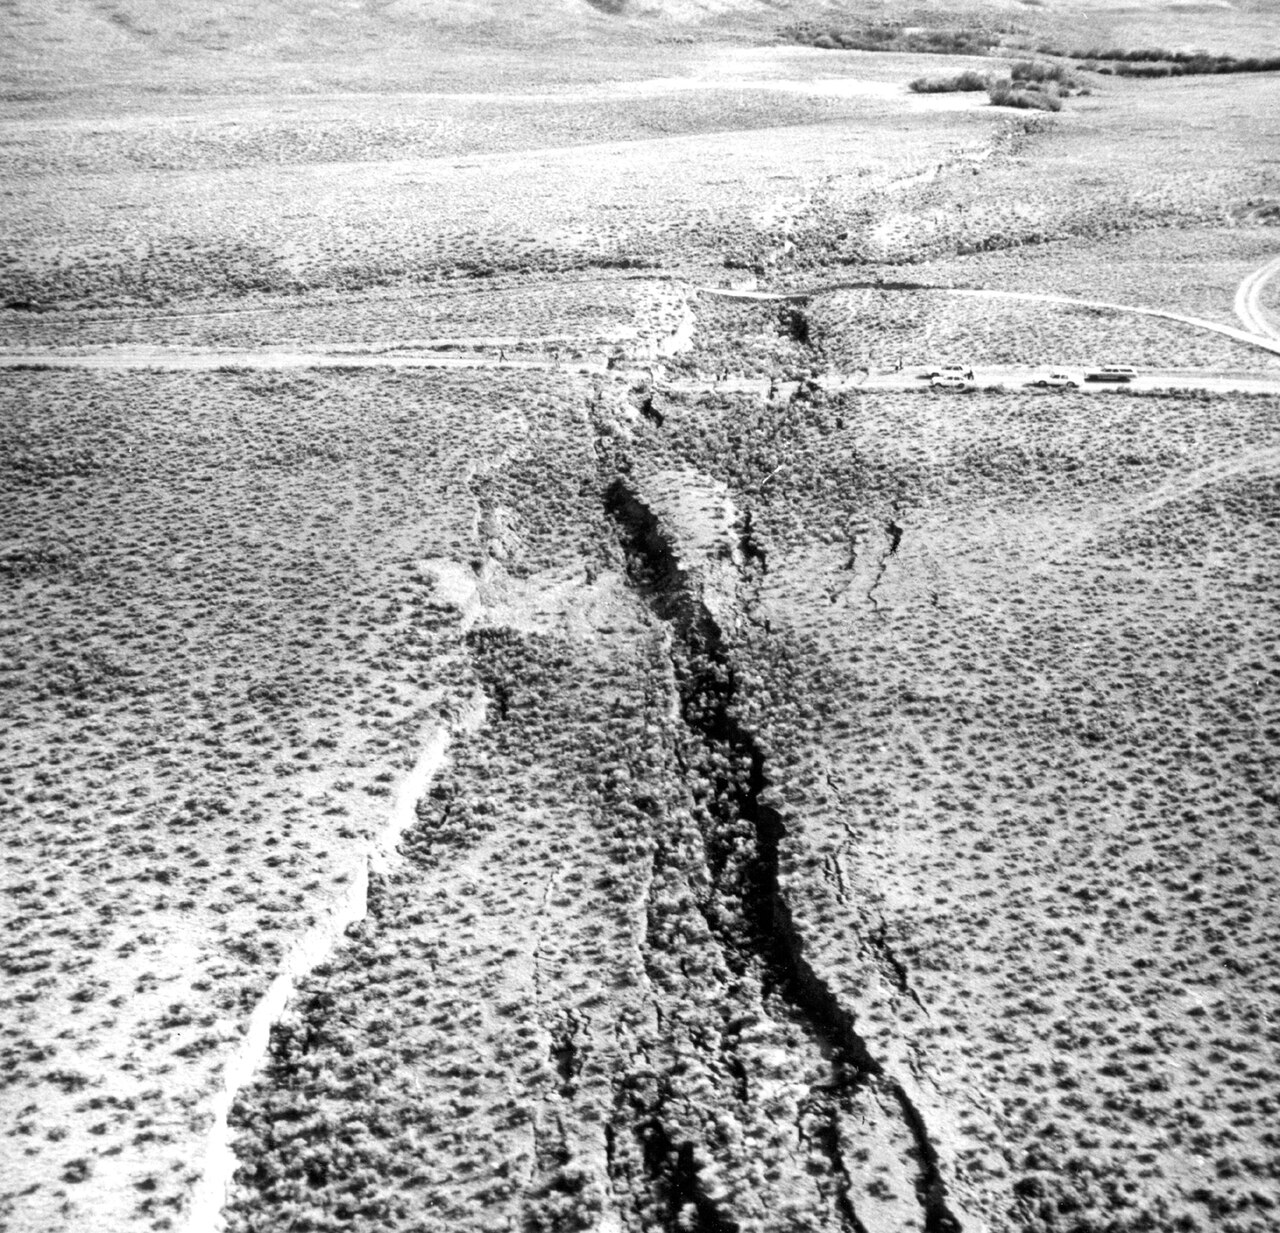
\includegraphics[width=0.62\linewidth]{images/book1/g7-borah-scarp.jpg}

{\small Treden in de grond die de \omterm{def:g4:volcanoes-earthquakes-first-look:earthquake}{aardbeving} van Borah Peak in 1983 in
Idaho (Verenigde Staten) achterliet, gezien vanuit de lucht: langs de
\omterm{def:g7:earthquakes:fault}{breuk} zakte de ene kant ten opzichte van de andere omlaag, en de trede
kruist bovenaan de weg. Foto: R.~E. Wallace, U.S. Geological Survey
(publiek domein, via Wikimedia Commons).}
% ledger: commons:borah-scarp
\label{fig:g7:earthquakes:borah}
\end{omfigure}

\begin{definition}[Haard en epicentrum]\label{def:g7:earthquakes:focus}
De \emph{haard}\index{haard} van een \omterm{def:g4:volcanoes-earthquakes-first-look:earthquake}{aardbeving} is de plek onder de grond,
op de \omterm{def:g7:earthquakes:fault}{breuk}, waar de verschuiving begint. Het
\emph{epicentrum}\index{epicentrum} is het punt aan het aardoppervlak
recht boven de haard.
\end{definition}

De \omterm{def:g7:earthquakes:focus}{haard} ligt vaak een paar kilometer tot een paar tientallen kilometers
diep. Van de 7\,031 \omterm{def:g4:volcanoes-earthquakes-first-look:earthquake}{aardbevingen} met \omterm{def:g7:earthquakes:magnitude}{magnitude}~6 of meer die tussen 1976 en
2025 zijn geregistreerd, hadden er 5\,561 --- 79~\% --- hun \omterm{def:g7:earthquakes:focus}{haard} op minder
dan \qty{70}{km} diepte. Maar 483 begonnen op meer dan \qty{300}{km}
diepte, en de diepste op \qty{688}{km}: deze diepe \omterm{def:g4:volcanoes-earthquakes-first-look:earthquake}{aardbevingen} vinden
plaats waar een \omterm{def:g7:plate-tectonics:plate}{plaat} onder een andere zakt, binnen de zakkende \omterm{def:g7:plate-tectonics:plate}{plaat}.
% ledger: data:usgs-comcat (figdata/grade-7/quake_counts.py, part depth)

Een grote \omterm{def:g4:volcanoes-earthquakes-first-look:earthquake}{aardbeving} komt zelden alleen. Vaak volgen er op dezelfde plek
kleinere, de \emph{naschokken}, wekenlang, maandenlang en zelfs jarenlang.
Soms gaan er kleinere \omterm{def:g4:volcanoes-earthquakes-first-look:earthquake}{aardbevingen} aan vooraf, maar niemand kan zeggen dat
het waarschuwingen waren voordat de grote heeft plaatsgevonden:
wetenschappers kunnen \omterm{def:g4:volcanoes-earthquakes-first-look:earthquake}{aardbevingen} niet voorspellen. Ze kunnen alleen
zeggen welke \omterm{def:g7:earthquakes:fault}{breuken} ooit opnieuw zullen verschuiven, en mensen helpen zich
voor te bereiden.
% ledger: usgs:eq-basics, usgs:seismograph

\begin{omfigure}
\begin{tikzpicture}[font=\small, x=1cm, y=1cm]
  % a block of crust seen in perspective: front face and top face
  \def\dx{2.2}\def\dy{1.3}
  % top surface: two blocks separated by the fault trace
  \fill[green!12] (0,0) -- (4.6,0) -- (4.6+\dx,\dy) -- (\dx,\dy) -- cycle;
  \fill[green!18] (4.6,0) -- (9,0) -- (9+\dx,\dy) -- (4.6+\dx,\dy) -- cycle;
  % front face
  \fill[brown!30] (0,0) -- (4.6,0) -- (3.4,-4) -- (0,-4) -- cycle;
  \fill[brown!40] (4.6,0) -- (9,0) -- (9,-4) -- (3.4,-4) -- cycle;
  % right face
  \fill[brown!22] (9,0) -- (9+\dx,\dy) -- (9+\dx,\dy-4) -- (9,-4) -- cycle;
  % fault plane on the front face and trace on top
  \draw[very thick, red!70!black] (4.6,0) -- (3.4,-4);
  \draw[very thick, red!70!black] (4.6,0) -- (4.6+\dx,\dy);
  % slip arrows
  \draw[-{Stealth[length=2.5mm]}, thick] (2.6,-0.35) -- (1.6,-0.35);
  \draw[-{Stealth[length=2.5mm]}, thick] (6.4,-0.35) -- (7.4,-0.35);
  \node[font=\footnotesize, anchor=south] at (2.1,-0.3) {blok 1};
  \node[font=\footnotesize, anchor=south] at (6.9,-0.3) {blok 2};
  % focus and waves
  \coordinate (F) at (3.95,-2.4);
  \foreach \r in {0.5,1.0,1.5,2.0}
    \draw[blue!60, dashed] (F) circle (\r);
  \fill[red!80!black] (F) circle (0.13);
  % epicentre: on the surface, straight above the focus (front edge of the top face)
  \coordinate (E) at (3.95,0);
  \draw[black!60, densely dotted, thick] (F) -- (E);
  \node[star, star points=5, star point ratio=2.4, fill=orange, draw=black, inner sep=1.4pt] at (E) {};
  % labels
  \node[anchor=west] at (9.5,-2.3) {haard};
  \draw[black!60] (9.45,-2.3) -- (4.1,-2.4);
  \node[anchor=south west] at (4.9,1.9) {epicentrum};
  \draw[black!60] (4.95,1.95) -- (4.05,0.12);
  \node[anchor=south, red!70!black] at (6.8,1.3) {breuk};
  \node[anchor=east, blue!60!black, align=right] at (-0.15,-2.6) {golven verspreiden\\zich in alle richtingen};
  \draw[blue!60, -{Stealth}] (-0.1,-2.6) -- (1.9,-2.5);
\end{tikzpicture}

{\small Een \omterm{def:g7:earthquakes:fault}{breuk}, de \omterm{def:g7:earthquakes:focus}{haard} en het \omterm{def:g7:earthquakes:focus}{epicentrum} (een tekening, niet op
schaal). De twee blokken schuiven langs de \omterm{def:g7:earthquakes:fault}{breuk} (rood) langs elkaar; de
verschuiving begint in de \omterm{def:g7:earthquakes:focus}{haard}, en van daaruit verspreiden golven zich in
alle richtingen, zoals rimpelingen op een vijver. Het \omterm{def:g7:earthquakes:focus}{epicentrum} (ster)
ligt aan het oppervlak, recht boven de \omterm{def:g7:earthquakes:focus}{haard}.}
% ledger: usgs:eq-basics
\label{fig:g7:earthquakes:fault}
\end{omfigure}


\section{Een aardbeving registreren}

\begin{definition}[Seismometer en seismogram]\label{def:g7:earthquakes:seismometer}
Een \emph{seismometer}\index{seismometer} is een instrument dat het schudden
van de grond registreert. Zijn registratie, een kronkelige lijn uitgezet
tegen de tijd, is een \emph{seismogram}\index{seismogram}.
\end{definition}

Het idee van een \omterm{def:g7:earthquakes:seismometer}{seismometer} is eenvoudig. Een frame is stevig aan de grond
bevestigd; daaraan hangt een zwaar gewicht aan een veer. Als de grond
schudt, schudt het frame mee, maar het zware gewicht, dat alleen door zijn
veer wordt vastgehouden, blijft bijna stil hangen. Het instrument
registreert de beweging van het frame ten opzichte van het stilhangende
gewicht: dat is de beweging van de grond. In de tekening hieronder schrijft
een pen die aan de massa vastzit die beweging op papier dat om een
draaiende trommel is gewikkeld.
% ledger: usgs:seismograph

\begin{omfigure}
\begin{tikzpicture}[font=\small, x=1cm, y=1cm]
  \begin{scope}
    % ground
    \fill[brown!30] (-0.6,-0.6) rectangle (5.0,0);
    \draw[decorate, decoration={snake, amplitude=1.2pt, segment length=6pt}, brown!70!black, thick]
      (-0.6,0) -- (5.0,0);
    % frame
    \fill[black!55] (0,0) rectangle (0.25,3.2);
    \fill[black!55] (0,3.0) rectangle (2.4,3.25);
    % spring and weight
    \draw[decorate, decoration={coil, aspect=0.5, segment length=3pt, amplitude=4pt}, thick]
      (2.1,3.0) -- (2.1,2.1);
    \fill[black!80] (1.7,1.45) rectangle (2.5,2.1);
    \node[white, font=\scriptsize] at (2.1,1.78) {massa};
    % pen arm and drum
    \draw[thick] (2.5,1.75) -- (3.45,1.75);
    \fill (3.45,1.75) circle (0.05);
    \draw[thick, fill=white] (3.95,1.75) circle (0.5);
    \draw[thick] (3.95,1.25) -- (3.95,0);
    \draw[-{Stealth}, black!60] (4.55,2.2) arc (40:-40:0.7);
    % labels
    \node[anchor=east, align=right, font=\footnotesize] at (-0.1,2.3) {frame vast\\aan de grond};
    \node[anchor=west, font=\footnotesize] at (2.6,2.65) {veer};
    \draw[black!60] (2.55,2.65) -- (2.25,2.6);
    \node[anchor=north, align=center, font=\footnotesize] at (2.1,1.35) {zware massa:\\blijft stil};
    \node[anchor=west, align=left, font=\footnotesize] at (4.7,1.05) {draaiende\\trommel\\met papier};
    \node[anchor=north, font=\footnotesize] at (2.2,-0.65) {de grond schudt};
  \end{scope}
  \begin{scope}[xshift=7.2cm, yshift=0.4cm]
    \begin{axis}[width=7.6cm, height=4.2cm, xmin=0, xmax=60, ymin=-1.1, ymax=1.1,
        axis x line=bottom, axis y line=none, xlabel={tijd (seconden)},
        tick label style={font=\scriptsize}, label style={font=\footnotesize}, clip=false]
      \addplot[black, line width=0.4pt] table[x=t, y=v] {figdata/out/grade-7-epicentre-m-trace.dat};
      \draw[blue!70!black, -{Stealth[length=2mm]}] (axis cs:10,1.45) -- (axis cs:10,0.45);
      \node[blue!70!black, font=\scriptsize, anchor=south east] at (axis cs:10.5,1.45) {snellere golven komen aan};
      \draw[red!70!black, -{Stealth[length=2mm]}] (axis cs:20,1.45) -- (axis cs:20,1.05);
      \node[red!70!black, font=\scriptsize, anchor=south west] at (axis cs:19.5,1.45) {tragere golven komen aan};
      \draw[{Stealth[length=2mm]}-{Stealth[length=2mm]}] (axis cs:10,-0.75) -- (axis cs:20,-0.75);
      \node[font=\scriptsize, anchor=east, align=right] at (axis cs:9,-0.75) {vertraging:\\10 s};
    \end{axis}
  \end{scope}
\end{tikzpicture}

{\small Links: het principe van een \omterm{def:g7:earthquakes:seismometer}{seismometer} (een tekening). Rechts: een
\omterm{def:g7:earthquakes:seismometer}{seismogram} dat voor dit boek is getekend (geen echte registratie): de lijn
is rustig, dan komen de snellere golven aan en tien seconden later de
tragere en grotere.}
% ledger: usgs:seismograph (trace drawn by figdata/grade-7/epicentre.py, part m-trace)
\label{fig:g7:earthquakes:seismometer}
\end{omfigure}

\subsection*{Hoe ver weg was de aardbeving?}

Een \omterm{def:g7:earthquakes:seismometer}{seismogram} vertelt meer dan ``de grond schudde''. De snellere golven
komen altijd eerst aan en de tragere daarna. Dicht bij de \omterm{def:g7:earthquakes:focus}{haard} komen ze
bijna tegelijk aan; ver weg raken de tragere golven steeds verder achter,
net zoals tijdens een onweer de donder verder achter de bliksem aan komt
als het onweer ver weg is. De vertraging tussen de twee aankomsten geeft
dus de afstand tot de \omterm{def:g4:volcanoes-earthquakes-first-look:earthquake}{aardbeving}.
% ledger: usgs:seismograph

Hoeveel kilometer voor elke seconde vertraging? Dat hangt af van de
snelheden van de twee golven in het \omterm{def:g3:stones-pebbles-sand:rock}{gesteente} dat ze doorkruisen. Met de
snelheden van het referentiemodel van de Aarde
(\cref{ch:g6:inside-the-earth}) betekent elke seconde vertraging ongeveer
\qty{7}{km} in de bovenste \omterm{def:g6:inside-the-earth:layers}{aardkorst} en \qty{9}{km} in de onderste
\omterm{def:g6:inside-the-earth:layers}{aardkorst}. In de oefeningen van dit hoofdstuk gebruiken we de ronde waarde
van \qty{8}{km} voor elke seconde.
% ledger: data:prem (computed in figdata/grade-7/epicentre.py, part rule)

\begin{method}[Het epicentrum vinden met drie stations]\label{met:g7:earthquakes:three-circles}
\begin{enumerate}
  \item Lees op het \omterm{def:g7:earthquakes:seismometer}{seismogram} van elk station de vertraging af tussen de
        aankomst van de snellere golven en de aankomst van de tragere.
  \item Zet elke vertraging om in een afstand (hier: $8 \times$ de
        vertraging in seconden, in kilometer).
  \item Teken op een \omterm{def:g2:drawing-to-map:map}{kaart} rond elk station een cirkel met als straal de
        afstand van dat station. Het \omterm{def:g7:earthquakes:focus}{epicentrum} ligt ergens op elke cirkel.
  \item Met twee cirkels zijn er meestal twee mogelijke punten; de derde
        cirkel gaat maar door een van beide: dat is het \omterm{def:g7:earthquakes:focus}{epicentrum}.
\end{enumerate}
\end{method}

\begin{example}[Drie cirkels]\label{ex:g7:earthquakes:three-circles}
Drie stations registreren dezelfde \omterm{def:g4:volcanoes-earthquakes-first-look:earthquake}{aardbeving}. De vertragingen zijn
\qty{10}{s} bij station~M1, \qty{11.25}{s} bij M2 en \qty{9.75}{s} bij M3.
De afstanden zijn $8 \times 10 = \qty{80}{km}$, $8 \times 11.25 = \qty{90}{km}$
en $8 \times 9.75 = \qty{78}{km}$. De drie cirkels, hieronder getekend,
snijden elkaar in één punt: het \omterm{def:g7:earthquakes:focus}{epicentrum}.
% ledger: usgs:seismograph (figdata/grade-7/epicentre.py, parts m-stations and m-circles)
\end{example}

\begin{omfigure}
\begin{tikzpicture}
  \begin{axis}[axis equal image, width=8.2cm, xmin=-150, xmax=170, ymin=-160, ymax=160,
      xtick={-120,-80,...,160}, ytick={-120,-80,...,120}, grid=both, grid style={black!12},
      tick label style={font=\scriptsize}, xlabel={km}, ylabel={km}, label style={font=\footnotesize}]
    \addplot[blue!60!black, line width=0.6pt] table[x=x, y=y] {figdata/out/grade-7-epicentre-m-circles.dat};
    \addplot[only marks, mark=triangle*, mark size=3pt, black,
        nodes near coords, point meta=explicit symbolic,
        nodes near coords style={font=\scriptsize, anchor=north, yshift=-2pt}]
      table[x=x, y=y, meta=name] {figdata/out/grade-7-epicentre-m-stations.dat};
    \node[star, star points=5, star point ratio=2.4, fill=orange, draw=black, inner sep=1.6pt] at (axis cs:0,0) {};
    \draw[black!60] (axis cs:-4,-4) -- (axis cs:-60,-75);
    \node[font=\scriptsize, anchor=north east, inner sep=1pt] at (axis cs:-60,-75) {epicentrum};
  \end{axis}
\end{tikzpicture}

{\small Elke cirkel heeft een station (driehoek) als middelpunt en als
straal de afstand van dat station tot de \omterm{def:g4:volcanoes-earthquakes-first-look:earthquake}{aardbeving}. De drie cirkels
snijden elkaar maar in één punt, het \omterm{def:g7:earthquakes:focus}{epicentrum} (ster).}
% ledger: usgs:seismograph (figdata/grade-7/epicentre.py, parts m-stations and m-circles)
\label{fig:g7:earthquakes:three-circles}
\end{omfigure}

\begin{omfigure}
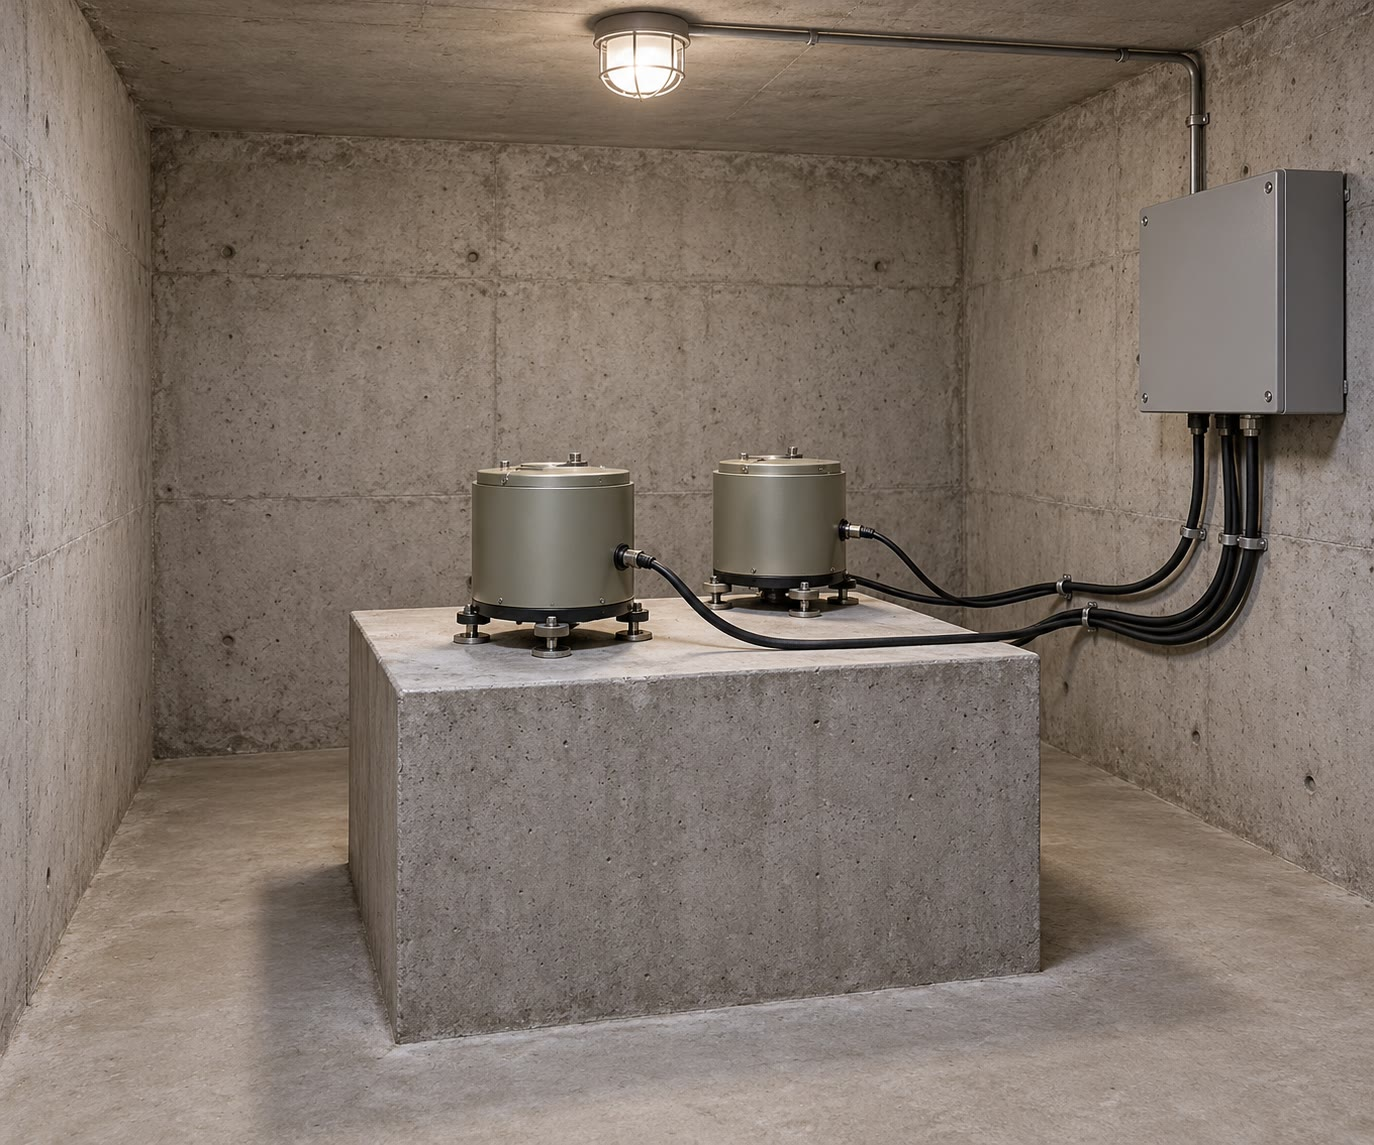
\includegraphics[width=0.58\linewidth]{images/book1/ai/g7-seismometer-vault.jpg}

{\small \omterm{def:g7:earthquakes:seismometer}{Seismometers} in een stille ondergrondse ruimte, op een betonnen
sokkel die op het \omterm{def:g3:stones-pebbles-sand:rock}{gesteente} rust, ver van wegen en machines (door AI
gegenereerde illustratie van een algemene scène).}
\label{fig:g7:earthquakes:vault}
\end{omfigure}

\section{Hoe groot? Magnitude en intensiteit}

Twee verschillende getallen beschrijven een \omterm{def:g4:volcanoes-earthquakes-first-look:earthquake}{aardbeving}, en ze worden vaak verward.

\begin{definition}[Magnitude]\label{def:g7:earthquakes:magnitude}
De \emph{magnitude}\index{magnitude} van een \omterm{def:g4:volcanoes-earthquakes-first-look:earthquake}{aardbeving} meet haar grootte:
de energie die bij de bron vrijkomt. Ze wordt uit de \omterm{def:g7:earthquakes:seismometer}{seismogrammen}
berekend. Elke \omterm{def:g4:volcanoes-earthquakes-first-look:earthquake}{aardbeving} heeft één enkele magnitude, geschreven met één
decimaal, zoals 6.3 of 9.1.
\end{definition}

\begin{definition}[Intensiteit]\label{def:g7:earthquakes:intensity}
De \emph{intensiteit}\index{intensiteit} van een \omterm{def:g4:volcanoes-earthquakes-first-look:earthquake}{aardbeving} op een plek
beschrijft hoe hevig de grond daar schudde, op basis van wat mensen voelden
en de schade die ze zagen. Ze wordt geschreven in Romeinse cijfers, van I
(niet gevoeld) tot XII (totale verwoesting). Eén \omterm{def:g4:volcanoes-earthquakes-first-look:earthquake}{aardbeving} heeft veel
intensiteiten: op elke plek een andere.
\end{definition}

De schaal van de magnitude stijgt snel. Elke stap van 1 in \omterm{def:g7:earthquakes:magnitude}{magnitude}
betekent golven die ongeveer 10~keer groter zijn op het \omterm{def:g7:earthquakes:seismometer}{seismogram} en
ongeveer 32~keer meer vrijgekomen energie. Een \omterm{def:g4:volcanoes-earthquakes-first-look:earthquake}{aardbeving} met \omterm{def:g7:earthquakes:magnitude}{magnitude}~8
maakt ongeveer $32 \times 32 \approx 1000$ keer meer energie vrij dan een
met \omterm{def:g7:earthquakes:magnitude}{magnitude}~6.
% ledger: usgs:mag-energy

\begin{method}[Twee magnitudes vergelijken]\label{met:g7:earthquakes:magnitudes}
Om de energie van twee \omterm{def:g4:volcanoes-earthquakes-first-look:earthquake}{aardbevingen} te vergelijken, tel je de hele stappen
tussen hun \omterm{def:g7:earthquakes:magnitude}{magnitudes} en vermenigvuldig je voor elke stap één keer met 32:
1~stap, 32~keer; 2~stappen, ongeveer 1000~keer; 3~stappen, ongeveer
32\,000~keer.
\end{method}

\begin{example}[Magnitude 9 en magnitude 7]\label{ex:g7:earthquakes:nine-seven}
De \omterm{def:g4:volcanoes-earthquakes-first-look:earthquake}{aardbeving} van 2004 voor de \omterm{def:g1:landscapes-around-us:water}{kust} van Sumatra had een \omterm{def:g7:earthquakes:magnitude}{magnitude} van 9.1.
Een \omterm{def:g4:volcanoes-earthquakes-first-look:earthquake}{aardbeving} met \omterm{def:g7:earthquakes:magnitude}{magnitude}~7.1 is twee stappen kleiner: ze maakte
ongeveer $32 \times 32 = 1024$, dus ongeveer 1000~keer, minder energie vrij.
% ledger: usgs:largest, usgs:mag-energy
\end{example}

De grootste \omterm{def:g4:volcanoes-earthquakes-first-look:earthquake}{aardbevingen} die ooit zijn gemeten, vonden allemaal plaats waar
een \omterm{def:g7:plate-tectonics:plate}{plaat} onder een andere zakt: \omterm{def:g7:earthquakes:magnitude}{magnitude}~9.5 in Chili op 22~mei 1960, 9.2
in Alaska in 1964, 9.1 voor de \omterm{def:g1:landscapes-around-us:water}{kust} van Sumatra in 2004 en 9.1 voor de \omterm{def:g1:landscapes-around-us:water}{kust}
van Japan op 11~maart 2011. Grote \omterm{def:g4:volcanoes-earthquakes-first-look:earthquake}{aardbevingen} zijn zeldzaam, en hoe groter
ze zijn, hoe zeldzamer, zoals het diagram laat zien: bij elke stap omhoog in
\omterm{def:g7:earthquakes:magnitude}{magnitude} ongeveer tien keer minder.
% ledger: usgs:largest, data:usgs-comcat

\begin{omfigure}
\begin{tikzpicture}
  \begin{axis}[ybar, width=0.72\linewidth, height=5.4cm, bar width=22pt,
      ymode=log, log origin y=infty, ymin=0.01, ymax=600,
      xtick=data, xticklabels={{6 tot 6.9},{7 tot 7.9},{8 tot 8.9},{9 of meer}},
      xlabel={magnitude}, ylabel={aardbevingen per jaar},
      ytick={0.01,0.1,1,10,100}, yticklabels={0.01,0.1,1,10,100},
      tick label style={font=\scriptsize}, label style={font=\small},
      nodes near coords, point meta=explicit symbolic,
      nodes near coords style={font=\scriptsize}, enlarge x limits=0.18,
      axis x line*=bottom, axis y line*=left]
    \addplot[fill=omThm!45, draw=omThm!80!black] table[x=cls, y=per_year, meta=per_year] {figdata/out/grade-7-quake_counts.dat};
  \end{axis}
\end{tikzpicture}

{\small \omterm{def:g4:volcanoes-earthquakes-first-look:earthquake}{Aardbevingen} per jaar, gemiddeld over 1976--2025, per \omterm{def:g7:earthquakes:magnitude}{magnitude}. De
verticale schaal is bijzonder: elke lijn staat voor tien keer zoveel als de
lijn eronder. Gegevens: aardbevingscatalogus van de U.S. Geological Survey
(7\,031 \omterm{def:g4:volcanoes-earthquakes-first-look:earthquake}{aardbevingen} met \omterm{def:g7:earthquakes:magnitude}{magnitude}~6 of meer).}
% ledger: data:usgs-comcat (figdata/grade-7/quake_counts.py, main table)
\label{fig:g7:earthquakes:counts}
\end{omfigure}

De intensiteitsschaal heeft geen formule: het is een lijst van wat er
gebeurt. De tabel geeft haar in verkorte vorm.
% ledger: usgs:mmi, usgs:mmi-page

\begin{center}
\small
\begin{tabular}{|c|p{0.8\linewidth}|}
\hline
\textbf{\omterm{def:g7:earthquakes:intensity}{intensiteit}} & \textbf{wat er gevoeld en gezien wordt} \\
\hline
I & niet gevoeld, behalve door heel enkele mensen \\
II & alleen gevoeld door enkele mensen in rust, vooral op hogere verdiepingen; hangende voorwerpen kunnen schommelen \\
III & binnenshuis gevoeld; het voelt als een voorbijrijdende vrachtwagen \\
IV & binnenshuis door velen gevoeld; servies, ramen en deuren rammelen \\
V & door bijna iedereen gevoeld, velen worden wakker; wat servies en enkele ramen breken \\
VI & door iedereen gevoeld, velen schrikken; wat zwaar meubilair verschuift; lichte schade \\
VII & weinig schade aan goed gebouwde gebouwen, veel aan slecht gebouwde; enkele schoorstenen breken \\
VIII & veel schade aan gewone gebouwen, sommige storten gedeeltelijk in; schoorstenen en muren vallen om \\
IX & grote schade, zelfs aan stevige gebouwen; gebouwen van hun fundering geschoven \\
X & de meeste gebouwen met hun fundering verwoest; rails verbogen \\
XI & weinig gebouwen blijven overeind; bruggen verwoest \\
XII & totale schade; voorwerpen de lucht in geworpen \\
\hline
\end{tabular}
\end{center}
% ledger: usgs:mmi

De \omterm{def:g7:earthquakes:intensity}{intensiteit} is meestal het hoogst bij het \omterm{def:g7:earthquakes:focus}{epicentrum} en neemt af met de
afstand. Maar ze hangt ook af van de ondergrond: \omterm{def:g3:stones-pebbles-sand:rock}{vast gesteente} schudt het
minst, zachte modder het meest. Een stad die op zachte grond is gebouwd,
kan harder schudden dan een andere stad die dichter bij het \omterm{def:g7:earthquakes:focus}{epicentrum} ligt
maar op \omterm{def:g3:stones-pebbles-sand:rock}{gesteente} is gebouwd.
% ledger: usgs:mag-energy

\begin{omfigure}
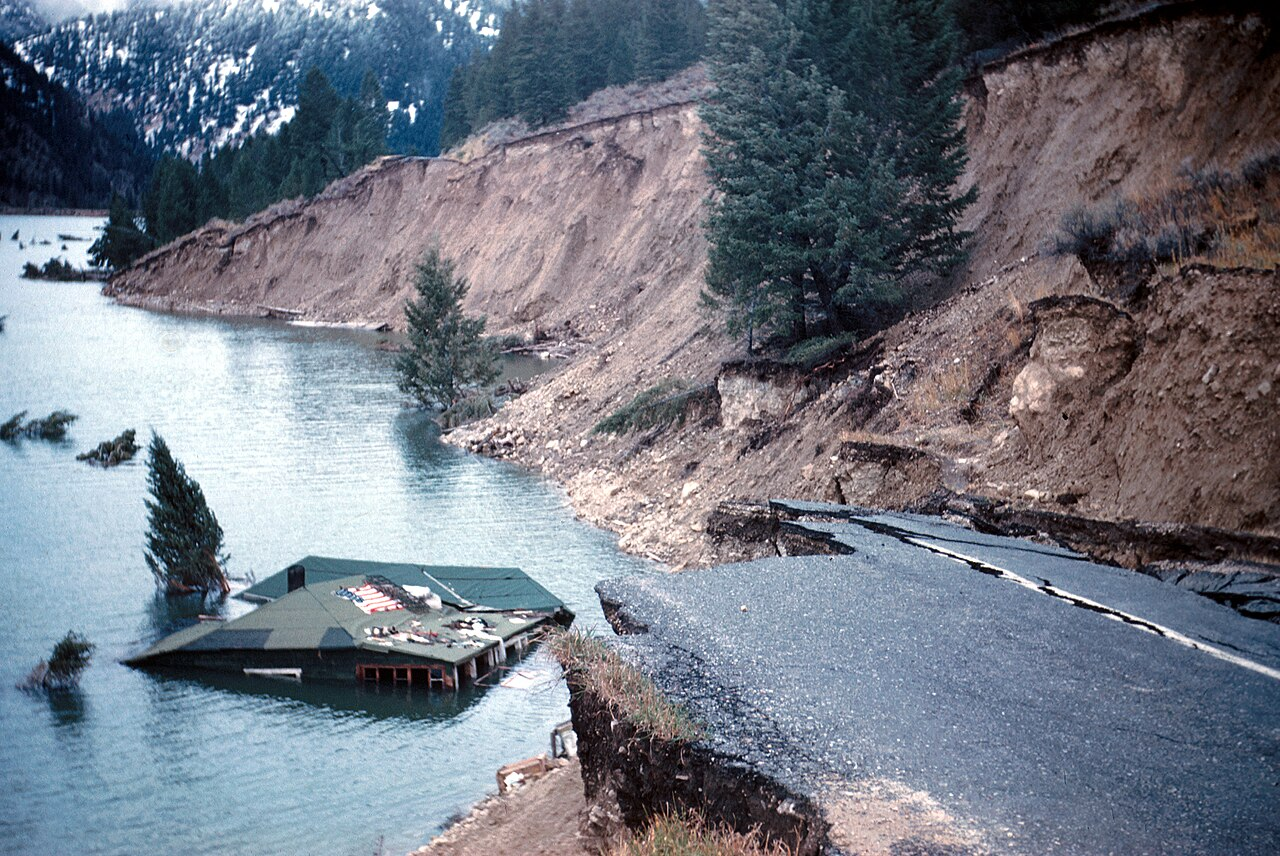
\includegraphics[width=0.6\linewidth]{images/book1/g7-hebgen-road.jpg}

{\small Na de \omterm{def:g4:volcanoes-earthquakes-first-look:earthquake}{aardbeving} bij Hebgen Lake, Montana (Verenigde Staten),
augustus 1959: de weg langs het \omterm{def:g1:landscapes-around-us:water}{meer} is in het water weggezakt, en een
lodge is bijna onder water komen te staan. Zulke schade is het kenmerk van
een hoge \omterm{def:g7:earthquakes:intensity}{intensiteit}. Foto: I.~J. Witkind, U.S. Geological Survey (publiek
domein, via Wikimedia Commons).}
% ledger: commons:hebgen-road, usgs:mmi
\label{fig:g7:earthquakes:hebgen}
\end{omfigure}

\section{Tsunami's}

\begin{definition}[Tsunami]\label{def:g7:earthquakes:tsunami}
Een \emph{tsunami}\index{tsunami} is een reeks zeegolven die op gang wordt
gebracht door een plotselinge beweging van de zeebodem --- meestal een
\omterm{def:g4:volcanoes-earthquakes-first-look:earthquake}{aardbeving} onder de \omterm{def:g2:water-on-earth:ocean}{zee}, soms een \omterm{def:g4:volcanoes-earthquakes-first-look:eruption}{uitbarsting} --- en die hele \omterm{def:g2:water-on-earth:ocean}{oceanen} kan
oversteken en de \omterm{def:g1:landscapes-around-us:water}{kusten} kan overstromen.
\end{definition}

Als een \omterm{def:g7:earthquakes:fault}{breuk} onder de \omterm{def:g2:water-on-earth:ocean}{zee} plotseling verschuift, beweegt de zeebodem
plotseling omhoog of omlaag, en tilt hij de hele waterkolom erboven op of
laat hij die zakken. Het water verspreidt zich in golven. Op de diepe
\omterm{def:g2:water-on-earth:ocean}{oceaan} is een \omterm{def:g7:earthquakes:tsunami}{tsunami} verrassend: hij is zelden hoger dan een meter, en
schepen merken niet eens dat hij onder hen door gaat. Maar hij is snel:
meer dan \qty{800}{km/h}, zo snel als een straalvliegtuig. Als hij ondiep
water bij de \omterm{def:g1:landscapes-around-us:water}{kust} bereikt, vertraagt hij tot 30 of \qty{50}{km/h} --- nog
altijd sneller dan iemand kan rennen --- en wordt hij hoger. De meeste
\omterm{def:g7:earthquakes:tsunami}{tsunami's} zijn bij de \omterm{def:g1:landscapes-around-us:water}{kust} minder dan \qty{3}{m} hoog; de grootste worden
meer dan \qty{30}{m}. De eerste golf is niet altijd de grootste, en de
golven kunnen urenlang blijven komen.
% ledger: nws:tsunami-speed, nws:tsunami-safety

\begin{omfigure}
\begin{tikzpicture}[font=\small, x=1cm, y=1cm]
  % sea floor profile: deep ocean on the left, shelf and coast on the right
  \fill[omSea!35] (0,0) -- (13.2,0) -- (13.2,-0.2) -- (11.4,-0.45) -- (10.2,-1.0) -- (8.8,-2.6) -- (0,-2.6) -- cycle;
  \fill[brown!35] (0,-2.6) -- (8.8,-2.6) -- (10.2,-1.0) -- (11.4,-0.45) -- (13.2,-0.2) -- (13.2,0.5) -- (14.2,1.0) -- (14.2,-3.3) -- (0,-3.3) -- cycle;
  % the broken fault under the sea, at left; one block lifted
  \draw[very thick, red!70!black] (1.9,-3.3) -- (2.3,-2.6);
  \draw[-{Stealth[length=2mm]}, thick] (2.75,-3.1) -- (2.75,-2.75);
  \node[anchor=north west, font=\footnotesize, red!70!black] at (0.1,-3.35) {de breuk verschuift, de zeebodem springt op};
  % wave: low and long in the deep ocean, short and tall near the coast
  \draw[blue!70!black, thick] (0,0) .. controls (1.2,0.18) and (2.2,0.18) .. (3.4,0)
     -- (5.0,0) .. controls (5.8,0.12) and (6.6,0.12) .. (7.4,0) -- (10.6,0)
     .. controls (11.0,0.55) and (11.6,0.9) .. (12.1,0) -- (13.2,0);
  \node[align=center, font=\footnotesize] at (2.0,0.85) {diepe oceaan: ongeveer 1 m hoog,\\meer dan 800 km/h};
  \node[align=center, font=\footnotesize] at (11.1,1.55) {bij de kust: trager\\(30 tot 50 km/h), veel hoger};
  \draw[-{Stealth[length=2.5mm]}, thick, blue!70!black] (4.4,0.45) -- (6.4,0.45);
  \node[font=\footnotesize] at (6.0,-1.5) {duizenden meters diep};
  \node[font=\footnotesize] at (12.0,-0.75) {ondiep};
\end{tikzpicture}

{\small Een \omterm{def:g7:earthquakes:tsunami}{tsunami} die de \omterm{def:g2:water-on-earth:ocean}{oceaan} oversteekt (een tekening, niet op schaal:
de hoogte van de golf is sterk overdreven). Boven de diepe \omterm{def:g2:water-on-earth:ocean}{oceaan} is hij
laag en heel snel; in ondiep water bij de \omterm{def:g1:landscapes-around-us:water}{kust} vertraagt hij en wordt hij
hoger.}
% ledger: nws:tsunami-speed
\label{fig:g7:earthquakes:tsunami}
\end{omfigure}

\begin{example}[Van Sumatra naar Sri Lanka]\label{ex:g7:earthquakes:colombo}
Colombo, de grootste stad van Sri Lanka, ligt ongeveer \qty{1830}{km} van het
\omterm{def:g7:earthquakes:focus}{epicentrum} van de \omterm{def:g4:volcanoes-earthquakes-first-look:earthquake}{aardbeving} van 2004. Met \qty{800}{km/h} legt een \omterm{def:g7:earthquakes:tsunami}{tsunami}
deze afstand af in $1830 \div 800 \approx 2.3$~uur, dat is ongeveer 2~uur
en 17~minuten. Niemand in Sri Lanka voelde de \omterm{def:g4:volcanoes-earthquakes-first-look:earthquake}{aardbeving}: de golf kwam
zonder enige andere waarschuwing dan die van de \omterm{def:g2:water-on-earth:ocean}{zee} zelf.
% ledger: nws:tsunami-speed, usgs:largest (distance and time in figdata/grade-7/quake_counts.py, part tsunami)
\end{example}

\begin{remark}[De waarschuwing die de zee geeft]\label{rem:g7:earthquakes:natural-warning}
% ledger: nws:tsunami-natural-warning, nws:tsunami-speed, shakeout:dch
Aan een \omterm{def:g1:landscapes-around-us:water}{kust} kunnen drie tekenen een \omterm{def:g7:earthquakes:tsunami}{tsunami} aankondigen: een sterke of
lange \omterm{def:g4:volcanoes-earthquakes-first-look:earthquake}{aardbeving}; de \omterm{def:g2:water-on-earth:ocean}{zee} die zich vreemd gedraagt --- een plotselinge
\omterm{def:g5:water-shapes-the-land:flood}{overstroming}, of water dat zich ver van de \omterm{def:g1:landscapes-around-us:water}{kust} terugtrekt en de zeebodem
blootlegt als bij heel laag tij; of een luid gebulder dat van de \omterm{def:g2:water-on-earth:ocean}{oceaan}
komt. Bescherm jezelf tijdens het schudden zoals je hebt geleerd (bukken,
dekken, vasthouden). Wacht daarna niet op een officiële waarschuwing: ga
meteen zo hoog, of zo ver landinwaarts, als je kunt. Een \omterm{def:g7:earthquakes:tsunami}{tsunami} van een
nabije \omterm{def:g4:volcanoes-earthquakes-first-look:earthquake}{aardbeving} kan binnen enkele minuten aankomen.
\end{remark}


\section{Oefeningen}

\begin{exercise}[$\star$]\label{exo:g7:earthquakes:1}
Koppel elk woord aan zijn betekenis: \omterm{def:g7:earthquakes:fault}{breuk}; \omterm{def:g7:earthquakes:focus}{haard}; \omterm{def:g7:earthquakes:focus}{epicentrum}; \omterm{def:g7:earthquakes:seismometer}{seismometer};
\omterm{def:g7:earthquakes:magnitude}{magnitude}; \omterm{def:g7:earthquakes:intensity}{intensiteit}. (a) De plek onder de grond waar de verschuiving
begint. (b) Hoe hevig de grond op één plek schudde. (c) Een scheur in het
\omterm{def:g3:stones-pebbles-sand:rock}{gesteente} waarlangs de twee kanten zijn verschoven. (d) Het punt aan het
oppervlak boven de \omterm{def:g7:earthquakes:focus}{haard}. (e) De grootte van een \omterm{def:g4:volcanoes-earthquakes-first-look:earthquake}{aardbeving}, één getal per
\omterm{def:g4:volcanoes-earthquakes-first-look:earthquake}{aardbeving}. (f) Een instrument dat het schudden van de grond registreert.
\end{exercise}

\begin{exercise}[$\star$]\label{exo:g7:earthquakes:2}
De \omterm{def:g7:earthquakes:focus}{haard} van een \omterm{def:g4:volcanoes-earthquakes-first-look:earthquake}{aardbeving} ligt \qty{30}{km} recht onder een dorp. (a)
Waar ligt het \omterm{def:g7:earthquakes:focus}{epicentrum}? (b) Hoe ver ligt het dorp van de \omterm{def:g7:earthquakes:focus}{haard}? (c) Een
tweede dorp ligt \qty{40}{km} van het \omterm{def:g7:earthquakes:focus}{epicentrum}. Zal de \omterm{def:g7:earthquakes:intensity}{intensiteit} daar
meestal hoger of lager zijn dan in het eerste dorp? Waarom?
\end{exercise}

\begin{exercise}[$\star$]\label{exo:g7:earthquakes:3}
\omterm{def:g7:earthquakes:magnitude}{Magnitude} of \omterm{def:g7:earthquakes:intensity}{intensiteit}? (a) ``De \omterm{def:g4:volcanoes-earthquakes-first-look:earthquake}{aardbeving} had een sterkte van 6.8.''
(b) ``In onze straat viel al het servies kapot en brak een schoorsteen.''
(c) ``Het was VI in de stad en IV in de dorpen in de \omterm{def:g1:landscapes-around-us:landform}{heuvels}.'' (d) ``Ze
maakte 32~keer meer energie vrij dan die van vorig jaar.''
\end{exercise}

\begin{exercise}[$\star$]\label{exo:g7:earthquakes:4}
Waar of niet waar? Verbeter de onware uitspraken. (a) Wetenschappers kunnen
een week van tevoren zeggen wanneer een \omterm{def:g4:volcanoes-earthquakes-first-look:earthquake}{aardbeving} zal toeslaan. (b) Op de
open \omterm{def:g2:water-on-earth:ocean}{oceaan} is een \omterm{def:g7:earthquakes:tsunami}{tsunami} een enorme muur van water. (c) Eén \omterm{def:g4:volcanoes-earthquakes-first-look:earthquake}{aardbeving}
heeft één enkele \omterm{def:g7:earthquakes:magnitude}{magnitude} maar veel \omterm{def:g7:earthquakes:intensity}{intensiteiten}. (d) De meeste grote
\omterm{def:g4:volcanoes-earthquakes-first-look:earthquake}{aardbevingen} vinden plaats in de buurt van \omterm{def:g7:plate-tectonics:plate-boundary}{plaatgrenzen}.
\end{exercise}

\begin{exercise}[$\star\star$]\label{exo:g7:earthquakes:5}
Gebruik het diagram van de \omterm{def:g4:volcanoes-earthquakes-first-look:earthquake}{aardbevingen} per jaar. (a) Ongeveer hoeveel
\omterm{def:g4:volcanoes-earthquakes-first-look:earthquake}{aardbevingen} met \omterm{def:g7:earthquakes:magnitude}{magnitude} 6 tot 6.9 vinden er in een jaar plaats? En met
\omterm{def:g7:earthquakes:magnitude}{magnitude} 7 tot 7.9? (b) Hoeveel keer minder zijn er van de tweede soort
dan van de eerste? (c) Tel de drie staven vanaf 7 op: ongeveer hoeveel
\omterm{def:g4:volcanoes-earthquakes-first-look:earthquake}{aardbevingen} met \omterm{def:g7:earthquakes:magnitude}{magnitude} 7 of meer vinden er in een jaar plaats? (d) Het
diagram geeft 0.04 per jaar voor \omterm{def:g7:earthquakes:magnitude}{magnitude} 9 of meer. Hoeveel is dat in
50~jaar?
\end{exercise}

\begin{exercise}[$\star\star$]\label{exo:g7:earthquakes:6}
Gebruik de methode om \omterm{def:g7:earthquakes:magnitude}{magnitudes} te vergelijken. (a) Hoeveel keer meer
energie maakt een \omterm{def:g4:volcanoes-earthquakes-first-look:earthquake}{aardbeving} met \omterm{def:g7:earthquakes:magnitude}{magnitude} 7 vrij dan een met \omterm{def:g7:earthquakes:magnitude}{magnitude} 6?
(b) En een met \omterm{def:g7:earthquakes:magnitude}{magnitude} 8 dan een met \omterm{def:g7:earthquakes:magnitude}{magnitude} 6? (c) Hoeveel keer
groter zijn de golven op het \omterm{def:g7:earthquakes:seismometer}{seismogram}, op dezelfde afstand, tussen
\omterm{def:g7:earthquakes:magnitude}{magnitude} 6 en 8?
\end{exercise}

\begin{exercise}[$\star\star$]\label{exo:g7:earthquakes:7}
Gebruik \qty{8}{km} voor elke seconde vertraging tussen de snellere en de
tragere golven. (a) Een station registreert een vertraging van \qty{5}{s}.
Hoe ver weg was de \omterm{def:g4:volcanoes-earthquakes-first-look:earthquake}{aardbeving}? (b) Een ander registreert \qty{25}{s}.
(c) Een \omterm{def:g4:volcanoes-earthquakes-first-look:earthquake}{aardbeving} vond plaats op \qty{120}{km} van een station: welke
vertraging leest het station af? (d) Waarom kan één station alleen niet
zeggen waar het \omterm{def:g7:earthquakes:focus}{epicentrum} ligt?
\end{exercise}

\begin{exercise}[$\star\star$]\label{exo:g7:earthquakes:8}
Gebruik de intensiteitstabel. Geef de \omterm{def:g7:earthquakes:intensity}{intensiteit} bij elk verslag. (a)
``Door bijna iedereen gevoeld; we werden wakker en er braken twee glazen.''
(b) ``Alleen mijn oma, die boven lag te rusten, voelde het; de lamp
schommelde.'' (c) ``Muren en schoorstenen vielen om; verscheidene huizen
stortten gedeeltelijk in.'' (d) Dezelfde \omterm{def:g4:volcanoes-earthquakes-first-look:earthquake}{aardbeving} leverde de verslagen
(a) en (c) op. Leg uit hoe dat mogelijk is.
\end{exercise}

\begin{exercise}[$\star\star$]\label{exo:g7:earthquakes:9}
Van de 7\,031 \omterm{def:g4:volcanoes-earthquakes-first-look:earthquake}{aardbevingen} met \omterm{def:g7:earthquakes:magnitude}{magnitude}~6 of meer uit 1976--2025 hadden
er 5\,561 hun \omterm{def:g7:earthquakes:focus}{haard} op minder dan \qty{70}{km} diepte. (a) Hoeveel hadden
een diepere \omterm{def:g7:earthquakes:focus}{haard}? (b) Welk percentage is dat? Rond af op een heel getal.
(c) De diepe vinden plaats waar een \omterm{def:g7:plate-tectonics:plate}{plaat} onder een andere zakt. Leg uit
waarom ze daar zo diep kunnen beginnen.
\end{exercise}

\begin{exercise}[$\star\star$]\label{exo:g7:earthquakes:10}
Malé, de hoofdstad van de Malediven, ligt ongeveer \qty{2500}{km} van het
\omterm{def:g7:earthquakes:focus}{epicentrum} van de \omterm{def:g4:volcanoes-earthquakes-first-look:earthquake}{aardbeving} van 2004. (a) Hoe lang deed de \omterm{def:g7:earthquakes:tsunami}{tsunami} er met
\qty{800}{km/h} over om de stad te bereiken? Geef uren en minuten.
(b) Hoeveel later kwam hij aan dan in Colombo (2~uur 17~minuten)?
(c) Waarom had een waarschuwingssysteem met zulke tijden veel levens kunnen
redden?
\end{exercise}

\begin{exercise}[$\star\star\star$]\label{exo:g7:earthquakes:11}
Een \omterm{def:g7:earthquakes:tsunami}{tsunami} legt \qty{400}{km} diepe \omterm{def:g2:water-on-earth:ocean}{oceaan} af met \qty{800}{km/h}, en
daarna de laatste \qty{20}{km} ondiep water met \qty{40}{km/h}. (a) Hoeveel
minuten doet hij over het diepe deel? (b) En over het ondiepe deel? (c) Hoe
lang duurt de hele tocht? (d) Wat is verrassend aan je antwoorden? (e)
Waarom wordt de golf hoger als hij vertraagt?
\end{exercise}

\begin{exercise}[$\star\star\star$]\label{exo:g7:earthquakes:12}
(a) Hoeveel keer meer energie maakt een \omterm{def:g4:volcanoes-earthquakes-first-look:earthquake}{aardbeving} met \omterm{def:g7:earthquakes:magnitude}{magnitude} 9 vrij dan
een met \omterm{def:g7:earthquakes:magnitude}{magnitude} 6? (b) Elk jaar zijn er ongeveer 127 \omterm{def:g4:volcanoes-earthquakes-first-look:earthquake}{aardbevingen} met
\omterm{def:g7:earthquakes:magnitude}{magnitude} 6 tot 6.9. Stel dat elk daarvan de energie van een \omterm{def:g7:earthquakes:magnitude}{magnitude} 6
vrijmaakt. Hoeveel jaar van zulke \omterm{def:g4:volcanoes-earthquakes-first-look:earthquake}{aardbevingen} is er nodig om de energie
van één \omterm{def:g4:volcanoes-earthquakes-first-look:earthquake}{aardbeving} met \omterm{def:g7:earthquakes:magnitude}{magnitude}~9 vrij te maken? (c) Wat zegt dit over het
aandeel van de energie dat de allergrootste \omterm{def:g4:volcanoes-earthquakes-first-look:earthquake}{aardbevingen} voor hun rekening
nemen?
\end{exercise}

\section{Probleem: Waar schudde de grond?}

\begin{problem}[{Weekendprobleem --- drie stations registreren een aardbeving
onder de zee, het epicentrum wordt op de kaart gevonden, en de stad Port
Hale wordt gewaarschuwd voordat de tsunami aankomt}]
\label{pb:g7:earthquakes:1}
% ledger: nws:tsunami-speed, usgs:seismograph, data:prem (figdata/grade-7/epicentre.py)
Onder de \omterm{def:g2:water-on-earth:ocean}{zee} voor een verzonnen \omterm{def:g1:landscapes-around-us:water}{kust} vindt een \omterm{def:g4:volcanoes-earthquakes-first-look:earthquake}{aardbeving} plaats. Drie
seismometerstations, A, B en C, staan op het land; de stad Port Hale ligt
op een eiland (\omterm{def:g2:drawing-to-map:map}{kaart} hieronder; één hokje is \qty{20}{km}). In deze streek
betekent elke seconde vertraging tussen de snellere en de tragere golven
\qty{8}{km}. De stations registreren:

\begin{center}
\small
\begin{tabular}{|c|c|c|}
\hline
\textbf{station} & \textbf{snellere golven komen aan} & \textbf{tragere golven komen aan} \\
\hline
A & 10:15:25 & 10:15:45 \\
B & 10:15:16 & 10:15:29 \\
C & 10:15:19 & 10:15:34 \\
\hline
\end{tabular}
\end{center}

\medskip
\noindent\textbf{Deel I --- Drie stations.}\par\nopagebreak
\begin{enumerate}[beginpenalty=10000]
  \item Bepaal voor elk station de vertraging tussen de twee aankomsten, in
        seconden.
  \item Welk station ligt het dichtst bij de \omterm{def:g4:volcanoes-earthquakes-first-look:earthquake}{aardbeving}? Hoe zie je dat
        zonder te rekenen?
  \item Bepaal de afstand van elk station tot de \omterm{def:g4:volcanoes-earthquakes-first-look:earthquake}{aardbeving}.
  \item De afstand van station A alleen zegt niet waar de \omterm{def:g4:volcanoes-earthquakes-first-look:earthquake}{aardbeving} was.
        Beschrijf alle plaatsen die op deze afstand van A liggen.
\end{enumerate}

\begin{center}
\begin{tikzpicture}
  \begin{axis}[axis equal image, width=12cm, xmin=-60, xmax=360, ymin=-200, ymax=260,
      xtick={-60,-40,...,360}, ytick={-200,-180,...,260}, xticklabels={}, yticklabels={},
      major tick length=0pt,
      axis background/.style={fill=omSea!25}, clip mode=individual]
    \addplot[fill=omLithAlluv, draw=black!50, line width=0.4pt] table[x=x, y=y] {figdata/out/grade-7-epicentre-p-west.dat};
    \addplot[fill=omLithAlluv, draw=black!50, line width=0.4pt] table[x=x, y=y] {figdata/out/grade-7-epicentre-p-north.dat};
    \addplot[fill=omLithAlluv, draw=black!50, line width=0.4pt] table[x=x, y=y] {figdata/out/grade-7-epicentre-p-island.dat};
    % the grid over land and sea, drawn before the labels
    \pgfplotsinvokeforeach{-40,-20,...,340}{\draw[black!15] (axis cs:#1,-200) -- (axis cs:#1,260);}
    \pgfplotsinvokeforeach{-180,-160,...,240}{\draw[black!15] (axis cs:-60,#1) -- (axis cs:360,#1);}
    \addplot[only marks, mark=triangle*, mark size=3.2pt, black,
        nodes near coords, point meta=explicit symbolic,
        nodes near coords style={font=\small\bfseries, anchor=south west}]
      table[x=x, y=y, meta=name] {figdata/out/grade-7-epicentre-p-stations.dat};
    \addplot[only marks, mark=square*, mark size=2.4pt, red!70!black,
        nodes near coords, point meta=explicit symbolic,
        nodes near coords style={font=\small, anchor=north east, fill=omSea!25, inner sep=1pt}]
      table[x=x, y=y, meta=name] {figdata/out/grade-7-epicentre-p-town.dat};
    \draw[-{Stealth[length=2.5mm]}, line width=0.8pt] (axis cs:330,200) -- (axis cs:330,245);
    \node[font=\scriptsize\bfseries, anchor=north] at (axis cs:330,200) {N};
    \node[font=\scriptsize, anchor=west, fill=omLithAlluv, inner sep=1pt] at (axis cs:170,240) {1 hokje = 20 km};
    \fill (axis cs:-60,-200) circle (1.5pt);
    \node[font=\small\bfseries, anchor=north east] at (axis cs:-60,-200) {O};
  \end{axis}
\end{tikzpicture}
\end{center}
% ledger: (invented map: figdata/grade-7/epicentre.py, parts p-west, p-north, p-island, p-stations, p-town)

\medskip
\noindent\textbf{Deel II --- Het epicentrum vinden.}\par\nopagebreak
\begin{enumerate}[resume, beginpenalty=10000]
  \item Eén hokje is \qty{20}{km}. Hoeveel hokjes is de straal van elke
        cirkel?
  \item De hoek O ligt linksonder op de \omterm{def:g2:drawing-to-map:map}{kaart}. Station C ligt 3~hokjes ten
        oosten en 14.5~hokjes ten noorden van O; als je 6~hokjes
        (\qty{120}{km}) recht naar het oosten van C gaat, kom je bij een
        punt~E. Controleer op de \omterm{def:g2:drawing-to-map:map}{kaart} dat E ook op de cirkels van A en B
        ligt: het is het \omterm{def:g7:earthquakes:focus}{epicentrum}. Hoeveel hokjes ten oosten en ten
        noorden van O ligt het?
  \item Ligt het \omterm{def:g7:earthquakes:focus}{epicentrum} op het land of onder de \omterm{def:g2:water-on-earth:ocean}{zee}? Waarom is dat van
        belang?
  \item De \omterm{def:g7:earthquakes:magnitude}{magnitude} was 7.4. Hoeveel keer meer energie dan een \omterm{def:g4:volcanoes-earthquakes-first-look:earthquake}{aardbeving}
        met \omterm{def:g7:earthquakes:magnitude}{magnitude}~6.4 maakte ze vrij?
\end{enumerate}

\medskip
\noindent\textbf{Deel III --- De golf bereikt de kust.}\par\nopagebreak
\begin{enumerate}[resume, beginpenalty=10000]
  \item Op de \omterm{def:g2:drawing-to-map:map}{kaart} ligt Port Hale 12~hokjes van het \omterm{def:g7:earthquakes:focus}{epicentrum}. Hoeveel
        kilometer is dat?
  \item Hoeveel minuten doet de \omterm{def:g7:earthquakes:tsunami}{tsunami} er met \qty{800}{km/h} over om Port
        Hale te bereiken?
  \item Het lokaliseren van de \omterm{def:g4:volcanoes-earthquakes-first-look:earthquake}{aardbeving} en het versturen van de
        waarschuwing duurt 5~minuten vanaf het begin van het schudden.
        Hoeveel tijd na de \omterm{def:g4:volcanoes-earthquakes-first-look:earthquake}{aardbeving} bereikt de waarschuwing Port Hale?
  \item Hoeveel minuten hebben de inwoners van Port Hale om hoger gelegen
        grond te bereiken voordat de \omterm{def:g7:earthquakes:tsunami}{tsunami} aankomt?
\end{enumerate}
\end{problem}
